% interactnlmsample.tex
% v1.05 - August 2017

\documentclass[]{interact}

\usepackage{epstopdf}% To incorporate .eps illustrations using PDFLaTeX, etc.
\usepackage[caption=false]{subfig}% Support for small, `sub' figures and tables
%\usepackage[nolists,tablesfirst]{endfloat}% To `separate' figures and tables from text if required
%\usepackage[doublespacing]{setspace}% To produce a `double spaced' document if required
%\setlength\parindent{24pt}% To increase paragraph indentation when line spacing is doubled

\usepackage{algorithm,algorithmic}
\usepackage{hyperref}
\usepackage{mathtools}
\usepackage{amssymb}
\usepackage{caption}
\usepackage{subcaption}
\usepackage{tikz}
\usepackage{multirow}
\usepackage{booktabs,tabularx}

\usepackage[numbers,sort&compress]{natbib}% Citation support using natbib.sty
\bibpunct[, ]{[}{]}{,}{n}{,}{,}% Citation support using natbib.sty
\renewcommand\bibfont{\fontsize{10}{12}\selectfont}% Bibliography support using natbib.sty
\makeatletter% @ becomes a letter
\def\NAT@def@citea{\def\@citea{\NAT@separator}}% Suppress spaces between citations using natbib.sty
\makeatother% @ becomes a symbol again

\theoremstyle{plain}% Theorem-like structures provided by amsthm.sty
\newtheorem{theorem}{Theorem}[section]
\newtheorem{lemma}[theorem]{Lemma}
\newtheorem{corollary}[theorem]{Corollary}
\newtheorem{proposition}[theorem]{Proposition}

\theoremstyle{definition}
\newtheorem{definition}[theorem]{Definition}
\newtheorem{example}[theorem]{Example}

\theoremstyle{remark}
\newtheorem{remark}{Remark}
\newtheorem{notation}{Notation}

\begin{document}

\articletype{ARTICLE TEMPLATE}% Specify the article type or omit as appropriate

\title{Taylor \& Francis \LaTeX\ template for authors (\textsf{Interact} layout + NLM reference style)}

\author{
\name{A.~N. Author\textsuperscript{a}\thanks{CONTACT A.~N. Author. Email: latex.helpdesk@tandf.co.uk} and John Smith\textsuperscript{b}}
\affil{\textsuperscript{a}Taylor \& Francis, 4 Park Square, Milton Park, Abingdon, UK; \textsuperscript{b}Institut f\"{u}r Informatik, Albert-Ludwigs-Universit\"{a}t, Freiburg, Germany}
}

\maketitle

\begin{abstract}
This template is for authors who are preparing a manuscript for a Taylor \& Francis journal using the \LaTeX\ document preparation system and the \texttt{interact} class file, which is available via selected journals' home pages on the Taylor \& Francis website.
\end{abstract}

\begin{keywords}
Sections; lists; figures; tables; mathematics; fonts; references; appendices
\end{keywords}


\section{Introduction}

In order to assist authors in the process of preparing a manuscript for a journal, the Taylor \& Francis `\textsf{Interact}' layout style has been implemented as a \LaTeXe\ class file based on the \texttt{article} document class. A \textsc{Bib}\TeX\ bibliography style file and a sample bibliography are also provided in order to assist with the formatting of your references.

Commands that differ from or are provided in addition to standard \LaTeXe\ are described in this document, which is \emph{not} a substitute for a \LaTeXe\ tutorial.

The \texttt{interactnlmsample.tex} file can be used as a template for a manuscript by cutting, pasting, inserting and deleting text as appropriate, using the preamble and the \LaTeX\ environments provided (e.g.\ \verb"\begin{abstract}", \verb"\begin{keywords}").


\subsection{The \textsf{Interact} class file}\label{class}

The \texttt{interact} class file preserves the standard \LaTeXe\ interface such that any document that can be produced using \texttt{article.cls} can also be produced with minimal alteration using the \texttt{interact} class file as described in this document.

If your article is accepted for publication it will be typeset as the journal requires in Minion Pro and/or Myriad Pro. Since most authors will not have these fonts installed, the page make-up is liable to alter slightly with the change of font. Also, the \texttt{interact} class file produces only single-column format, which is preferred for peer review and will be converted to two-column format by the typesetter if necessary during preparation of the proofs. Please therefore do not try to match the typeset format exactly, but use the standard \LaTeX\ fonts instead and ignore details such as slightly long lines of text or figures/tables not appearing in exact synchronization with their citations in the text: these details will be dealt with by the typesetter. Similarly, it is unnecessary to spend time addressing warnings in the log file -- if your .tex file compiles to produce a PDF document that correctly shows how you wish your paper to appear, such warnings will not prevent your source files being imported into the typesetter's program.


\subsection{Submission of manuscripts prepared using \emph{\LaTeX}}

Manuscripts for possible publication should be submitted to the Editors for review as directed in the journal's Instructions for Authors, and in accordance with any technical instructions provided in the journal's ScholarOne Manuscripts or Editorial Manager site. Your \LaTeX\ source file(s), the class file and any graphics files will be required in addition to the final PDF version when final, revised versions of accepted manuscripts are submitted.

Please ensure that any author-defined macros used in your article are gathered together in the preamble of your .tex file, i.e.\ before the \verb"\begin{document}" command. Note that if serious problems are encountered in the coding of a document (missing author-defined macros, for example), the typesetter may resort to rekeying it.


\section{Benchmark Desription}
The LRA benchmark employs two energy groups and two delayed precursors and represents a 2-D quarter-core, BWR model subject to a control-rod ejection with adiabatic heating \cite{anl}.
Schematic layout of the problem is shown in Fig.~\ref{fig:lra core}, where region numbers indicate different materials and region R is the ejected rod.
%To produce time-dependent snapshots, the deterministic transport code Detran\footnote{https://github.com/robertsj/libdetran} was used to solve the time-dependent diffusion equations.
\begin{figure}[h!]
	\centering
	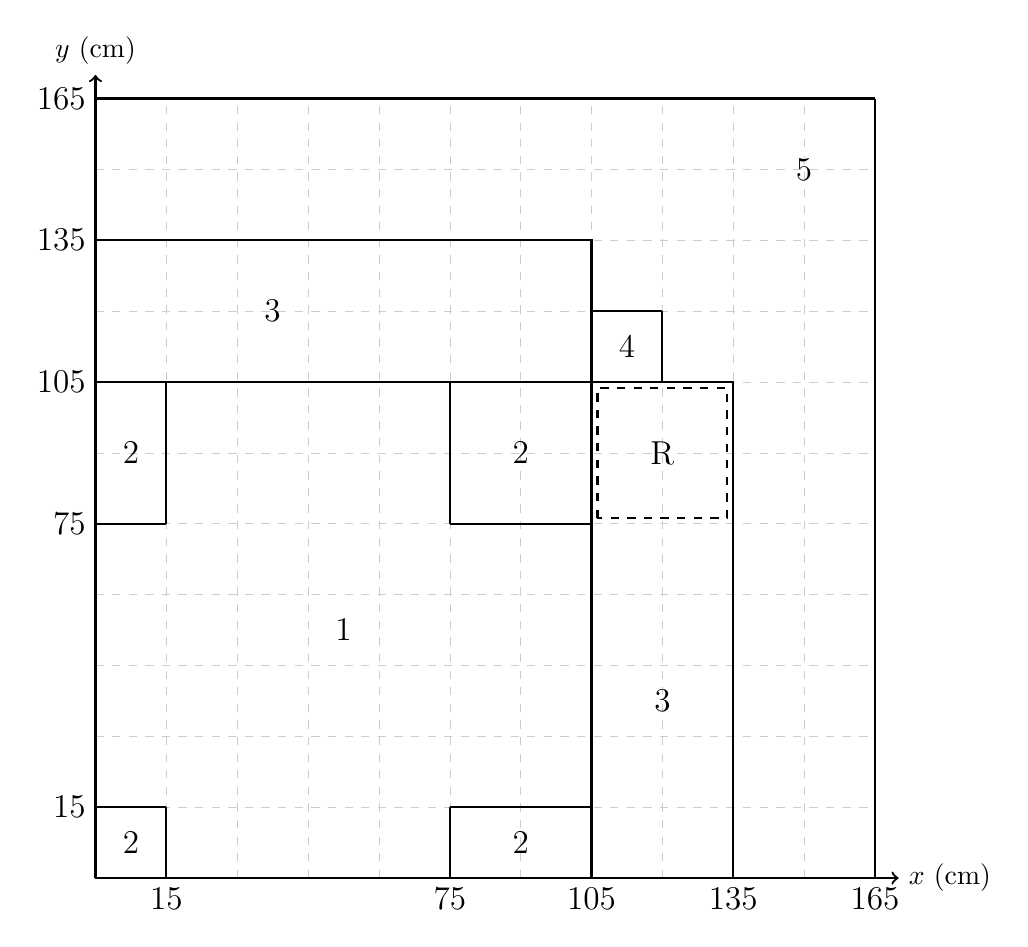
\begin{tikzpicture}[scale=0.6]	
	\begin{scope}<->;
	
	% GRID
	\draw[step=1.5cm,gray,very thin, dashed,opacity=0.4] (0, 0) grid (16.5,16.5);
	
	% AXES
	\draw[black, thick, ->] (0, 0) -- (17,  0) node[right] {$x$ (cm)};
	\draw[black, thick, ->] (0, 0) -- ( 0, 17) node[above] {$y$ (cm)};
	
	% Material 1 regions 
	
	\node[font=\large] at (5.25, 5.25) {1};
	
	% Material 2 regions
	\draw[black, thick] (0, 1.5) -- (1.5, 1.5);
	\draw[black, thick] (1.5, 0) -- (1.5, 1.5);
	\node[font=\large] at (0.75, 0.75) {2};
	
	\draw[black, thick] ( 7.5, 0.0) -- ( 7.5, 1.5);
	\draw[black, thick] (10.5, 0.0) -- (10.5, 1.5);
	\draw[black, thick] ( 7.5, 1.5) -- (10.5, 1.5);
	\node[font=\large] at (9.0, 0.75) {2};
	
	\draw[black, thick] ( 0.0,  7.5) -- ( 1.5,  7.5);
	\draw[black, thick] ( 0.0, 10.5) -- ( 1.5, 10.5);
	\draw[black, thick] ( 1.5,  7.5) -- ( 1.5, 10.5);
	\node[font=\large] at ( 0.75, 9.0) {2};
	
	\draw[black, thick] ( 7.5,  7.5) -- ( 7.5, 10.5);
	\draw[black, thick] ( 7.5,  7.5) -- (10.5,  7.5);
	\draw[black, thick] (10.5, 10.5) -- ( 7.5, 10.5);
	\draw[black, thick] (10.5, 10.5) -- (10.5,  7.5);
	\node[font=\large] at ( 9.0, 9.0) {2};
	
	% Material 3 regions
	\draw[black, thick] (10.5,  0.0) -- (10.5, 10.5) -- (13.5, 10.5) --  (13.5,  0.0) -- (10.5,  0.0);
	\node[font=\large] at ( 12.0, 3.75) {3}; 
	\draw[black, thick] (0.0, 10.5) -- (10.5, 10.5) -- (10.5, 13.5) -- (0.0, 13.5) --  (0.0, 10.5);
	\node[font=\large] at ( 3.75, 12.0) {3}; 
	
	% Material 4 regions  
	\draw[black, thick] ( 12,  12) -- ( 12, 10.5) -- (10.5, 10.5) -- (10.5,  12) -- ( 12,  12);
	\node[font=\large] at ( 11.25,11.25) {4};
	
	
	% Material 5 regions
	\draw[black, thick] ( 16.5,  0.0) -- (16.5, 16.5);
	\draw[black, thick] (  0.0, 16.5) -- (16.5, 16.5);
	\node[font=\large] at (15.0, 15.0) {5};
	
	% Perturbed regions
	\def\eps{0.125}
	\draw[black, thick, dashed] (10.5+\eps, 7.5+\eps) -- (10.5+\eps, 10.5-\eps) -- (13.5-\eps, 10.5-\eps) -- (13.5-\eps, 7.5+\eps) --  (10.5+\eps, 7.5+\eps);
	
	\node[font=\large] at (12,9) {R};
	
	% ticks
	\foreach \x/\xtext in {15, 75, 105, 135, 165}
	\draw[black,xshift=0.1*\x cm] (0,.3) -- (0,0) node[below, font=\large] {$\xtext$};
	\foreach \y/\ytext in {15, 75, 105, 135, 165}
	\draw[black,yshift=0.1*\y cm] (.3,0) -- (0,0) node[left, font=\large] {$\ytext$};
	\end{scope}
	\end{tikzpicture}
	\caption{Schematic of LRA benchmark.}
	\label{fig:lra core}
\end{figure}
The transient is initiated by a control rod ejection with constant velocity over a period of 2 seconds leading to a super-critical prompt transient, in which the power increased by about 10 orders of magnitude in a very short time.
The control rod movement was simulated by changing the thermal absorption cross section of the control rod material.
\begin{equation}
\sigma 
\end{equation}

Thermal feedback is incorporated through adiabatic fuel heat-up defined by
\begin{equation}
\frac{\partial}{\partial t}T(x,t) = \alpha[\Sigma_{f1}(x,t)\phi_1(x,t)+\Sigma_{f2}(x,t)\phi_2(x,t)] \, ,
\label{eq:heatup}
\end{equation}
and corresponding Doppler feedback defined by
\begin{equation}
\Sigma_{a1}(x,t) = \Sigma_{a1}(x,t=0)[1+\gamma(\sqrt{(T(x,t)}-\sqrt{(T_0)})] \, ,
\label{eq:doppler}
\end{equation}
where $\Sigma_{f_i}$ is the fission cross section of group $i$, $T$ is the temperature,  $\Sigma_{a1}$ is the fast absorption cross section and  $T_0$ is the initial temperature which is $300 $ K,
$\alpha = 3.83\times 10^{-11}~\text{K}.\text{cm}^3$ and $\gamma = 3.034\times 10^{-3} ~\text{K}^{-0.5}$.\\
The power is computed as
\begin{equation}
P(x,t)=\kappa [\Sigma_{f1}(x,t)\phi_1(x,t)+\Sigma_{f2}(x,t)\phi_2(x,t)] \, ,
\end{equation}
where $\kappa = 3.204\times 10^{-11}~ \text{Ws/fission}$.
The model was implemented in the deterministic transport code Detran~\cite{roberts2014advanced}.  
A mesh-centered, finite-volume discretization was used for the spatial dicretization, while a first-order, backward-difference temporal discretization was used with a fixed 0.001 s step size.  
The initial condition for the transient was computed by solving the steady-state equation, for which the $k_{\text{eff}}$ was found to be 0.9975.
Note that at each time step the fast absorption cross section is a function of the solution itself, hence a fixed point non-linear iteration is employed.
A convergence criteria is used such that the $\text{L}_2$ norm  of the relative flux error between two consecutive iterations is less than $1\times 10^{-6}$,

\begin{equation}
\|\frac{\mathbf{\Phi}^{i+1} - \mathbf{\Phi}^{i}} {\mathbf{\Phi}^i}\| \le  1\times 10^{-6} \, , 
\end{equation}
where the superscript $i$ denotes the iteration number.
The transient was calculated for 3.0 seconds.
Figure~\ref{fig:lra fom power} shows the reference full-order model power along with the core average temperature, while Figure \ref{fig:lra ss flux} shows the steady state group flux distribution.
This reference solution is not numerically converged in either the space or the time but it represents the simulation response that one wish to approximate.
\begin{figure}[h!]
	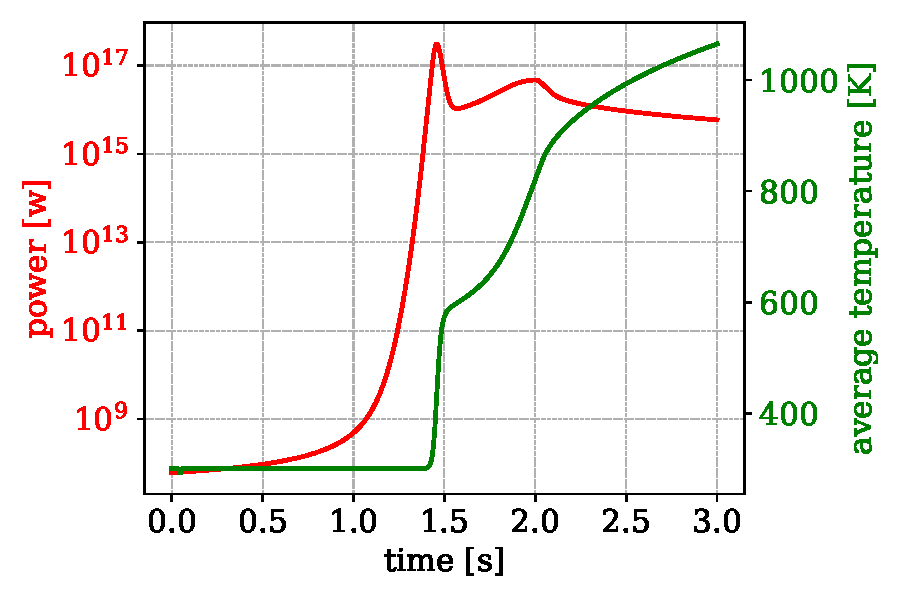
\includegraphics[width=1.0\linewidth]{../figures/LRA_fom_power_temperature.pdf}
	\caption{LRA core power}
	\label{fig:lra fom power}
\end{figure}

\begin{figure}[H]
	\centering
	\begin{subfigure}[b]{0.7\textwidth}
		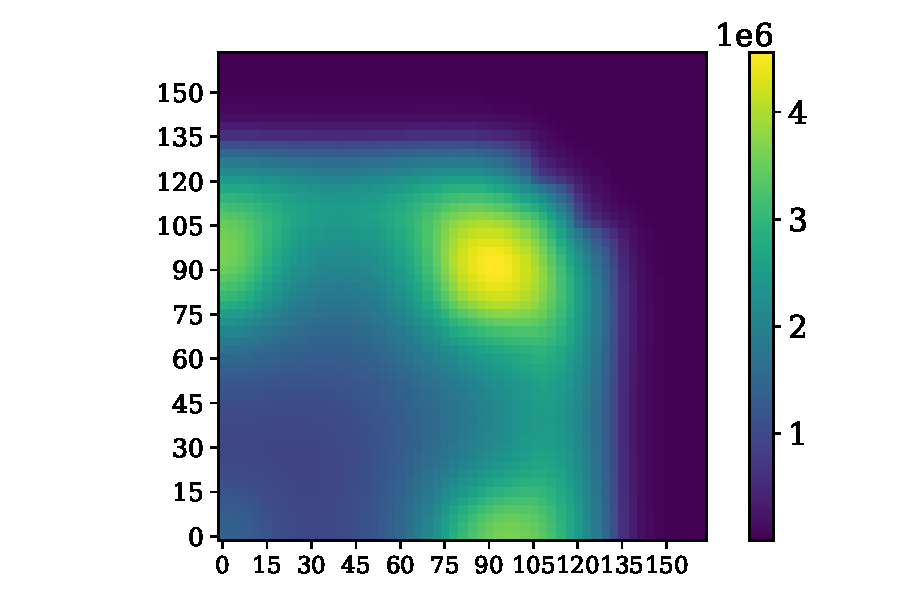
\includegraphics[width=1.0\linewidth]{../figures/ss_fom_fast_flux_image.pdf}
		\caption{Steady state fast flux.}
		\label{fig:ss fast flux}
	\end{subfigure}
	\begin{subfigure}[b]{0.7\textwidth}
		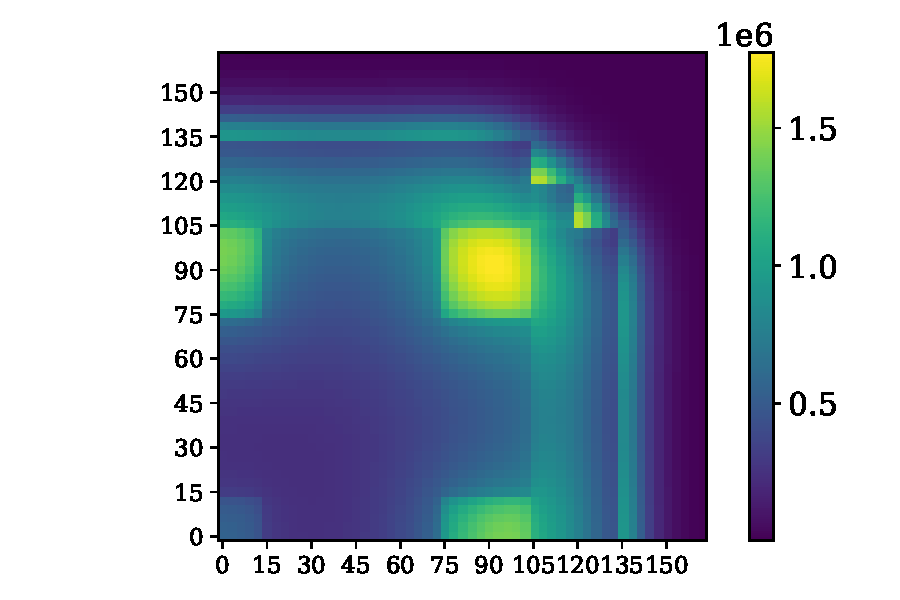
\includegraphics[width=1.0\linewidth]{../figures/ss_fom_thermal_flux_image.pdf}
		\caption{Steady state thermal flux.}
		\label{fig:ss thermal flux}
	\end{subfigure}
	\caption{Steady state group flux $(\text{neutrons}.\text{cm}^2/s)$}
	\label{fig:lra ss flux}
\end{figure}


\begin{table}[h!]
	\centering
	\begin{tabular}{l|l|l|l| l|l}
		material & group  & $D$ (cm) & $\Sigma_{a} ~ (\text{cm}^{-1})$ & $\Sigma_{s2\gets 1}~ (\text{cm}^{-1})$ & $\nu\Sigma_{f}~ (\text{cm}^{-1})$ \\\hline
		\multirow{2}{*}{1}& 1   & 1.255  &  0.008252   &  \multirow{2}{*}{0.02533} & 0.004602 \\	
		& 2   & 0.211  &  0.1003     &           & 0.1091  \\
		\hline
		
		\multirow{2}{*}{2}& 1   & 1.268  &  0.007181    & \multirow{2}{*}{0.02767} & 0.004609 \\	
		& 2   & 0.1902 &  0.07047     &           &  0.08675\\
		\hline
		
		\multirow{2}{*}{3}& 1   & 1.259  &  0.008002    & \multirow{2}{*}{0.02617}     & 0.004663 \\	
		& 2   & 0.2091 &  0.08344     &    &    0.1021 \\
		\hline
		\multirow{2}{*}{4}& 1   & 1.259  &  0.008002    & \multirow{2}{*}{0.02617}  &  0.004663 \\	
		& 2   & 0.2091 &  0.073324    &           &  0.1021   \\
		\hline
		\multirow{2}{*}{5}& 1   & 1.257  &  0.0006034   &  \multirow{2}{*}{0.04754}  & 0.0 \\	
		& 2   & 0.1592 &   0.01911    &        & 0.0 \\
		\hline
	\end{tabular}
	{\raggedright $v_1 = 3\times10^{7} ~\text{cm/sec}. $,  $v_2 = ~3\times10^{5} \text{cm.sec}.$  \par}
	\caption{Two-group diffusion constants}
	\label{tab:twogroup}
\end{table}


\begin{table}[h!]
	\centering
	\begin{tabular}{c|l|l}
		group & $\beta_i$  & $\lambda_i$ ($s^{-1}$)  \\
		\hline
		1    &  0.0054 & 0.00654 \\
		2    &  0.001087 & 1.35  \\
		\hline
	\end{tabular}
	\caption{Delayed neutron data.}
	\label{tab:precursor data}
\end{table}


\section{ROM}
\subsection{ROM Implementation}

Using the POD-Galerkin projection, a ROM was constructed to approximate the group flux and the core power of the LRA benchmark.
As discussed in the previous chapter, the time-dependent diffusion equation coupled with the precursors group equation can be cast into a compact form as in Eq.~\ref{eq:transient fom}.
Similar to the TWIGL benchmark ROM, POD basis set was generated for each group flux while one basis set was generated for both precursors groups, i.e, 
$\mathbf{\Phi}_1(t) = \mathbf{U}_1\mathbf{a}_1(t)$, $\mathbf{\Phi}(t)_2 = \mathbf{U}_2\mathbf{a}_2(t)$ and $\mathbf{C}(t) = \mathbf{U}_c\mathbf{a}_c(t)$, where the $\mathbf{U}_1$, $\mathbf{U}_2$  and $\mathbf{U}_c$ are the POD bases of the fast group, thermal group and precursor concentration respectively, and $\mathbf{a}_1$, $\mathbf{a}_2$ and $\mathbf{a}_c$ are their respective temporal coefficients. 
The first 100 normalized singular values \footnote{The normalization is done be dividing each singular value by the sum of all singular values.} of the group flux are shown in Fig.~\ref{fig:lra singular values}.
\begin{figure}[h!]
	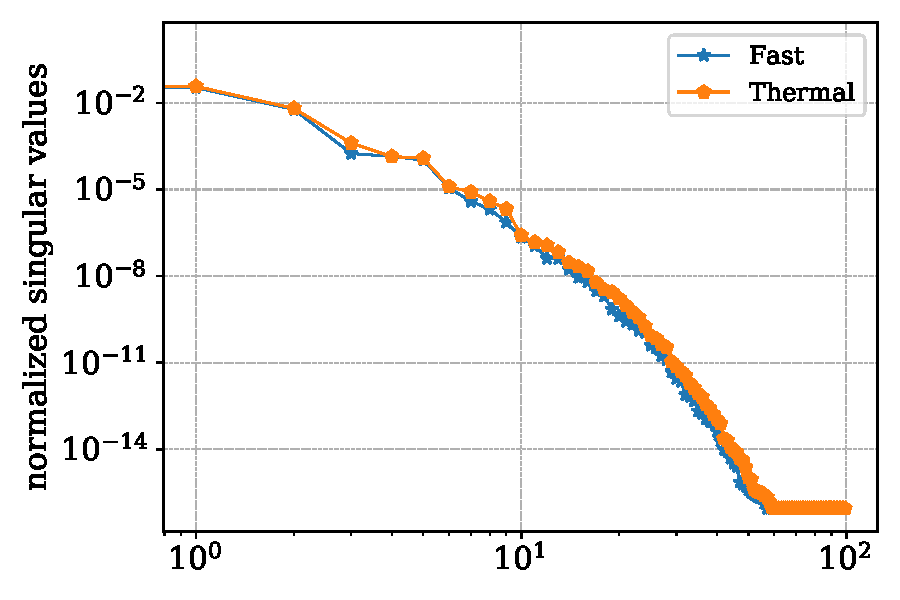
\includegraphics[width=1.0\linewidth]{figures/LRA/LRA_singular_values.pdf}
	\caption{flux normalized singular value.}
	\label{fig:lra singular values}
\end{figure}
Since the focus of this application is on treating the non-linearity, rather than trying different ranks of the POD basis, rank 30 was chosen for each group flux and for the precursor concentration.
Also, the temperature field was approximated by projecting it onto a lower dimensional POD space
\begin{equation}
\mathbf{T}(t) = \mathbf{U}_{\text{temp}}\mathbf{a}_T(t) \, ,
\label{eq:temp pod}
\end{equation}
where $\mathbf{U}_{\text{temp}}\in\mathbb{R}^{n \times r_T} $ is the POD subspace of rank $r_T$ and $\mathbf{a}_T\in \mathbb{R}^{r_T}$ is a vector of the corresponding temporal coefficients. 
To obtain the subspace, snapshots of the temperature were collected at different times for which the SVD was computed.
Shown in Fig.~\ref{fig:lra T singular values} are the first 100 normalized singular values, based on which a POD of rank $10$ was selected for approximating the temperature.
\begin{figure}[H]
	\centering
	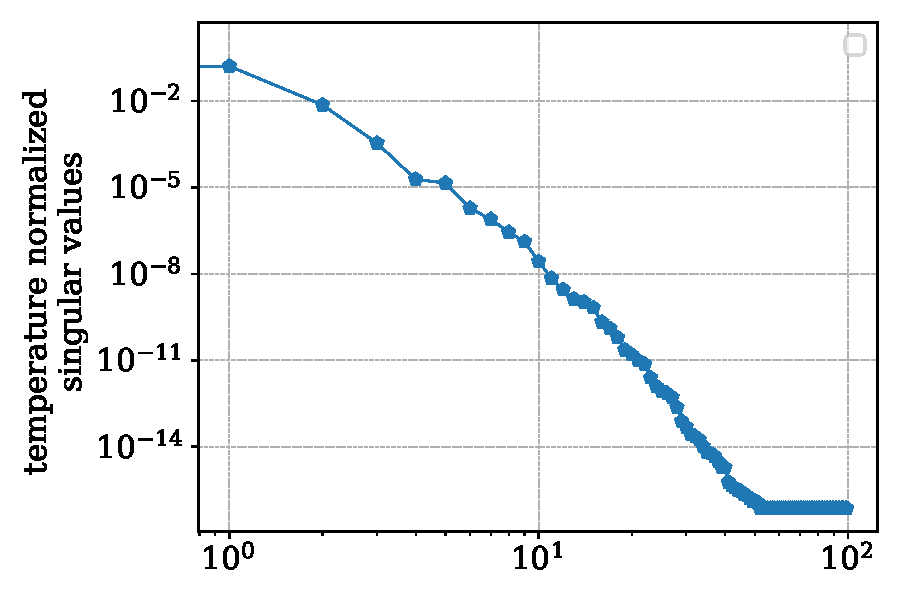
\includegraphics[width=1.0\linewidth]{figures/LRA/LRA_T_singular_values.pdf}
	\caption{temperature normalized singular value.}
	\label{fig:lra T singular values}
\end{figure}
Inserting Eq.~\ref{eq:temp pod} into Eq.~\ref{eq:heatup} and multiplying on the left by $\mathbf{U}_T^T$ \footnote{The superscript T denotes the matrix transpose.} yields
\begin{equation}
\frac{d\mathbf{a}_T(t)}{dt}  = \alpha [\underbrace{\mathbf{U}_{\text{temp}}^T \boldsymbol{\Sigma}_{f1}\mathbf{U}_1}_{\mathbf{U}_{T1}}\mathbf{a_1}(t) + \underbrace{\mathbf{U}_{\text{temp}}^T\boldsymbol{\Sigma}_{f2}\mathbf{U}_2}_{\mathbf{U}_{T2}}\mathbf{a_2}(t)] \, .
\label{eq:reduced temp}
\end{equation}
Note that $\mathbf{U}_{T1}$ and $\mathbf{U}_{T2}$ are time-independent, so they can be precomputed once and stored.
Thus, at each time step the flux temporal coefficients (i.e, $\mathbf{a_1}(t)$ and $\mathbf{a_2}(t)$) are computed by solving the reduced system and then used to compute the temperature coefficients by employing a first-order, backward-difference scheme to Eq.~\ref{eq:reduced temp}.
Similar to the full-order model, a fixed point iteration is used to treat the flux non-linearity.
However, it was observed that the reduced model needed more iterations to converge which could be due to the small value of some of the flux coefficients, hence a convergence criteria was employed based on the relative $\text{L}_2$ norm of the error of flux coefficients between two consecutive iterations 
\begin{equation}
\frac{\| \mathbf{a}^{i-1} - \mathbf{a}^{i}\|}{\|\mathbf{a}_i \|} \le 1\times 10^{-6}  \, , 
\end{equation}
Note that the fast absorption cross section needs to be updated at each time step using Eq.~\ref{eq:doppler} in which the core temperature distribution is required.
In order to avoid reconstructing the full order temperature, 
the DEIM was used to approximate the absorption cross section.
For this purpose, snapshots of which were collected in order to generate a POD subspace that is used to approximate its space and to find a set of interpolation indices as illustrated in Algorithm~\ref{alg:DEIM}.
DEIM of order $10$ was used and hence, the cross section was reconstructed at each time step at only 10 points in the spatial space.
Moreover, since the reactivity insertion was simulated by changing the absorption cross section, the operator $\mathbf{A}$ in Eq.~\ref{Eq:transient rom} exhibits time dependence, 
The MDEIM was used to decompose the operator and hence avoid performing the expensive projection at each time step.
Shown in Fig.~\ref{fig:lra L singular values} are the singular values resulting from the SVD of the serialized operator snapshots. 
Based on the shown plot, a DEIM of order $15$ was used.
\begin{figure}[H]
	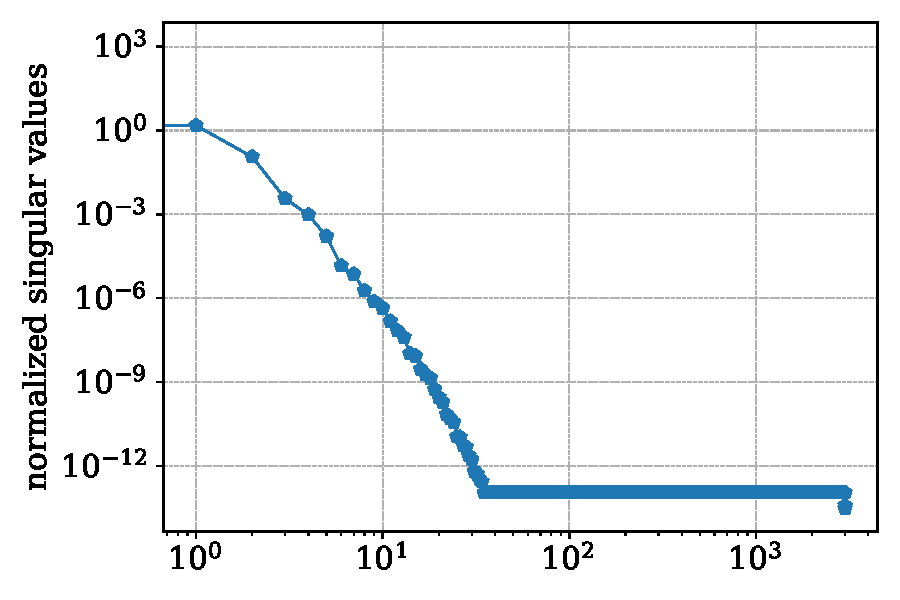
\includegraphics[width=1.0\linewidth]{figures/LRA/LRA_L_singular_values.pdf}
	\caption{Operator normalized singular value.}
	\label{fig:lra L singular values}
\end{figure}

%------------------------------------------------------------------------%
\subsection{Results}

\subsubsection{ROM results}
ROMs were constructed for FOMs models with increasing the spatial fidelity, i.e, spatial grids of $22\times 22$, $44\times44$ and $55 \times 55$.
For brevity, we show the POD modes with their temporal coefficients of only the $55 \times 55$  grid in Fig.~\ref{fig:lra flux modes}.
\begin{figure}[H]
	\centering
	\begin{subfigure}[b]{0.45\textwidth}
		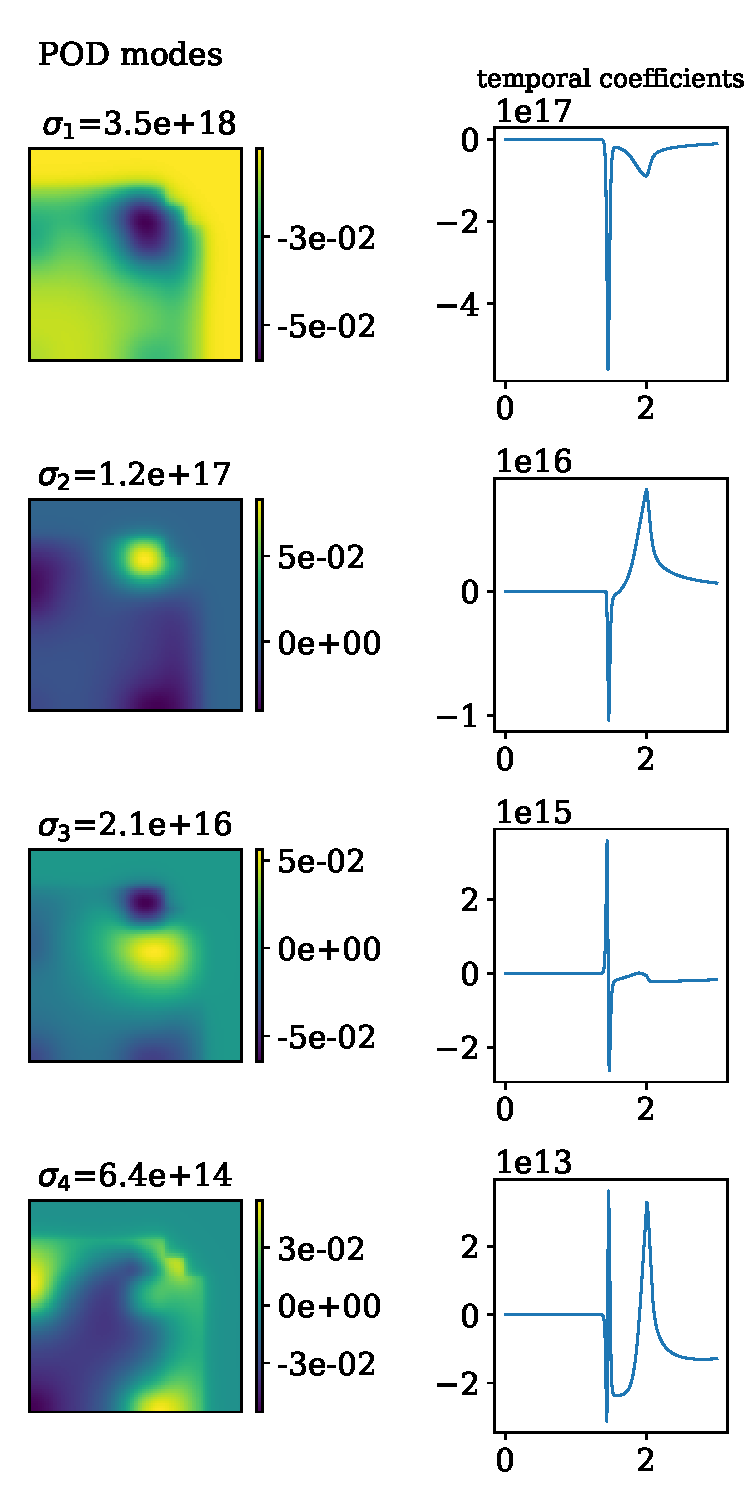
\includegraphics[width=1.0\linewidth]{../figures/LRA_fast_modes.pdf}
		\caption{Fast flux modes.}
		\label{fig:ss fast flux}
	\end{subfigure}
	\begin{subfigure}[b]{0.45\textwidth}
		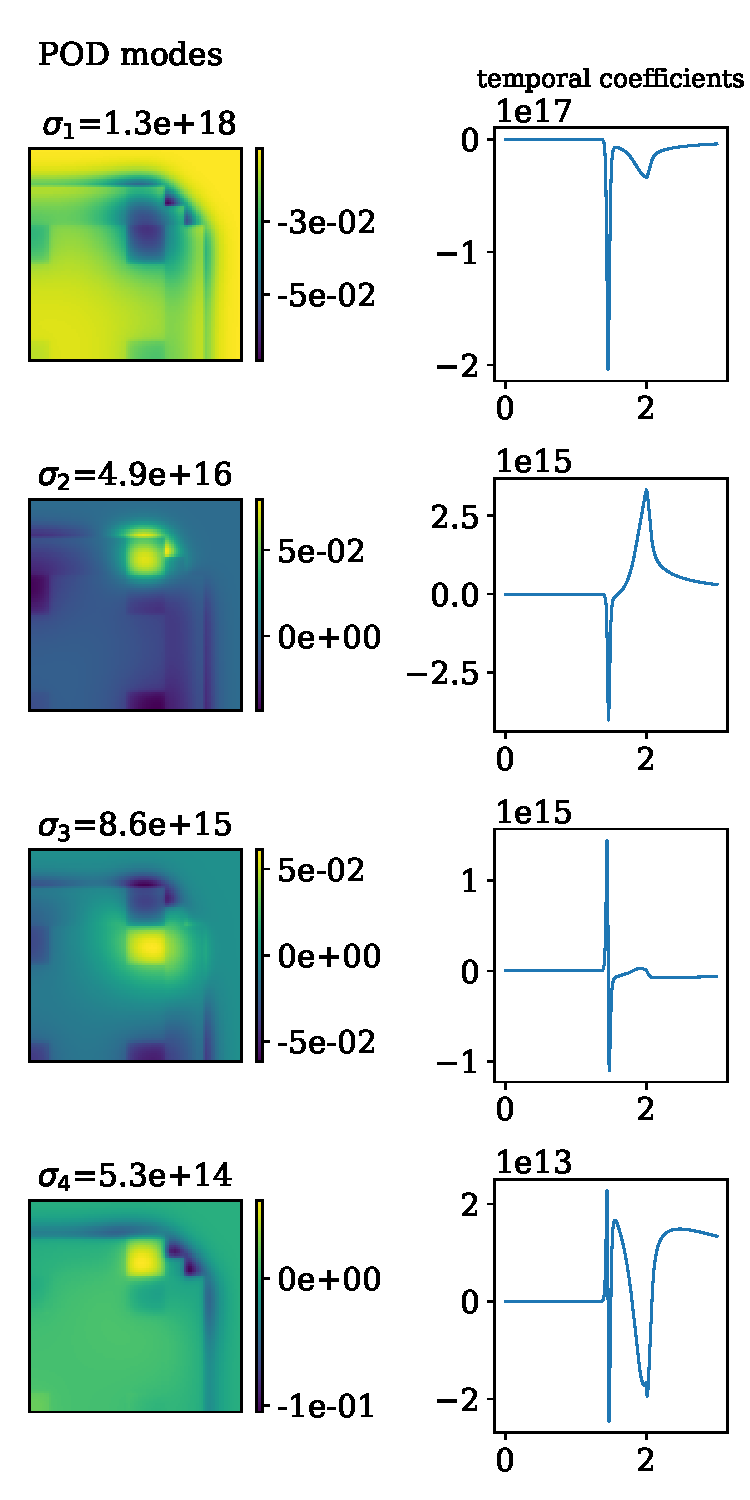
\includegraphics[width=1.0\linewidth]{../figures/LRA_thermal_modes.pdf}
		\caption{Thermal flux modes.}
		\label{fig:ss thermal flux}
	\end{subfigure}
	\caption{Flux POD modes and their temporal coefficient.}
	\label{fig:lra flux modes}
\end{figure}
Using ROMs with the specifications given in the previous section, the absolute relative error in the predicted powers are computed as shown in Fig.~\ref{fig:deim power error}.
\begin{figure}[H]
	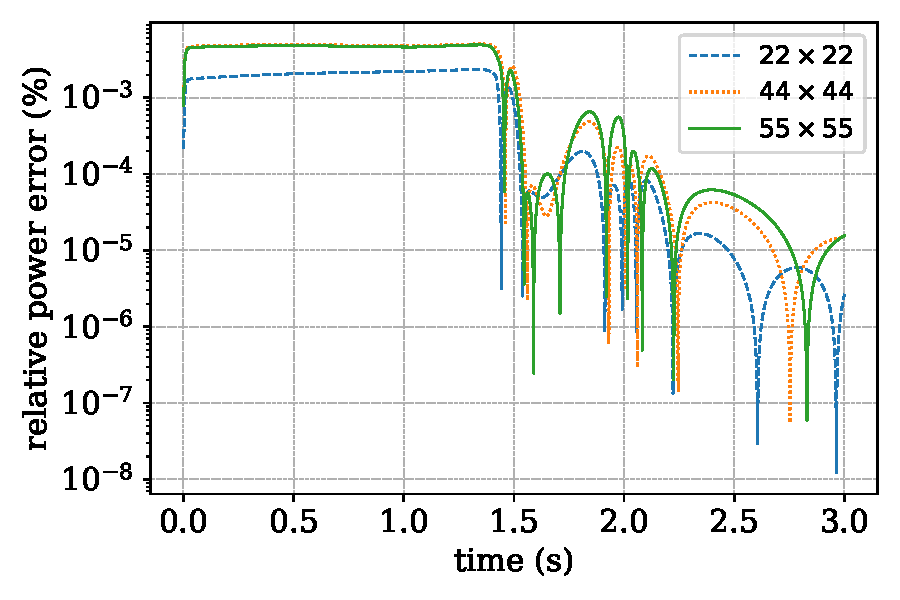
\includegraphics[width=1.0\linewidth]{../figures/LRA_power_deim_relative_error.pdf}
	\caption{Relative error of the power predicted by MDEIM ROM}
	\label{fig:deim power error}
\end{figure}
The maximum flux errors for both groups are shown in Table \ref{tab:lra flux errors}.

\begin{table*}[H]
	\centering
	\begin{tabular}{c|c|c}  
		grid &	fast flux  &  thermal flux \\
		\hline
		$22\times 22$ &    &  1     \\
		$44\times 44$ &    &       \\
		$55\times 55$ &    &       \\
		\hline
	\end{tabular}
	\caption{\bf maximum flux error of the fast and thermal flux (\%)}
	\label{tab:lra flux errors}
\end{table*}
It was interesting to compare the power error with that of a ROM without MDEIM, i.e, with performing the operator projection at each time step.
The power error is shown in Fig.~\ref{fig:rom power error} and apparently, the accuracy is comparable to that in Fig.~\ref{fig:deim power error}, implying an accurate approximation of the problem operator via the MDEIM. 
\begin{figure}[H]
	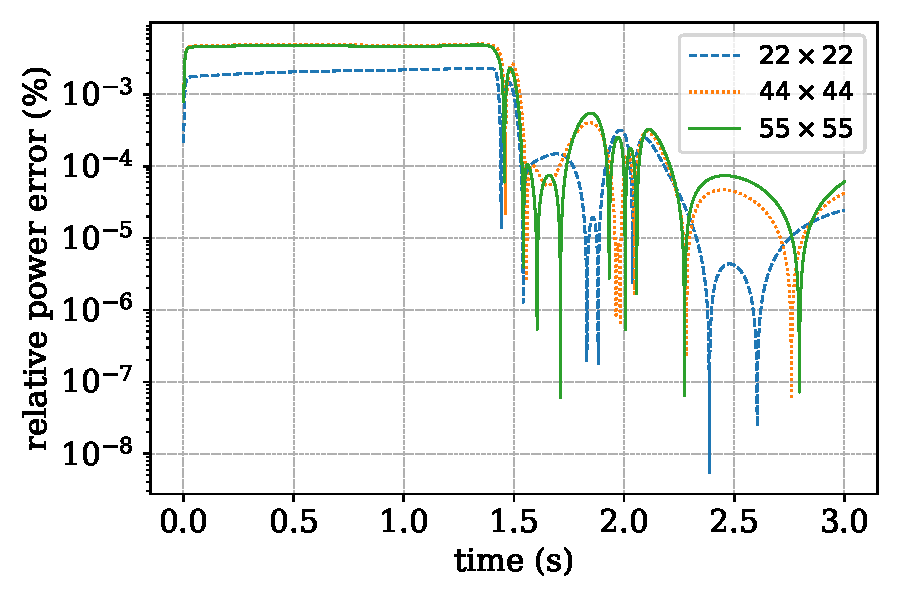
\includegraphics[width=1.0\linewidth]{../figures/LRA_power_rom_relative_error.pdf}
	\caption{Relative error of the power predicted by ROM.}
	\label{fig:rom power error}
\end{figure}
Also, the spatial-averaged relative error in the approximated temperature was computed and is shown in Fig.~\ref{fig:deim tempearture error}.
\begin{figure}[H]
	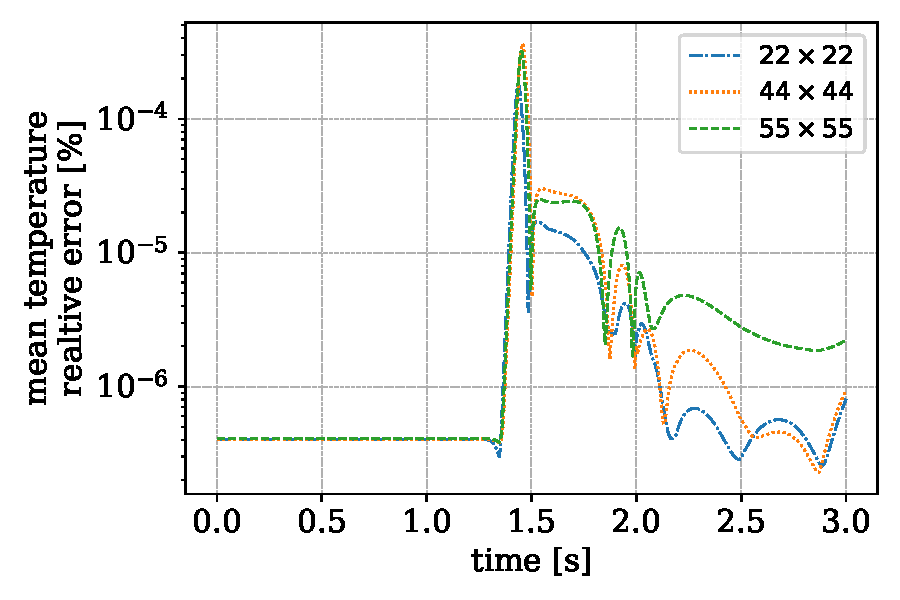
\includegraphics[width=1.0\linewidth]{../figures/temperature_relative_error.pdf}
	\caption{Relative error of the temperature predicted by ROM.}
	\label{fig:deim tempearture error}
\end{figure}

As mentioned earlier, the non-linearity of the fast absorption cross section was approximated using DEIM of rank 10.
Shown in Fig.~\ref{fig:cross-section deim indices} are the 10 selected interpolation points on the absorption cross section map at the last time step. i.e, $t=3$ s.
Thus, the temperature is constructed only at these locations from which the cross section is evaluated using Eq.~\ref{eq:doppler}.

\begin{figure}[H]
	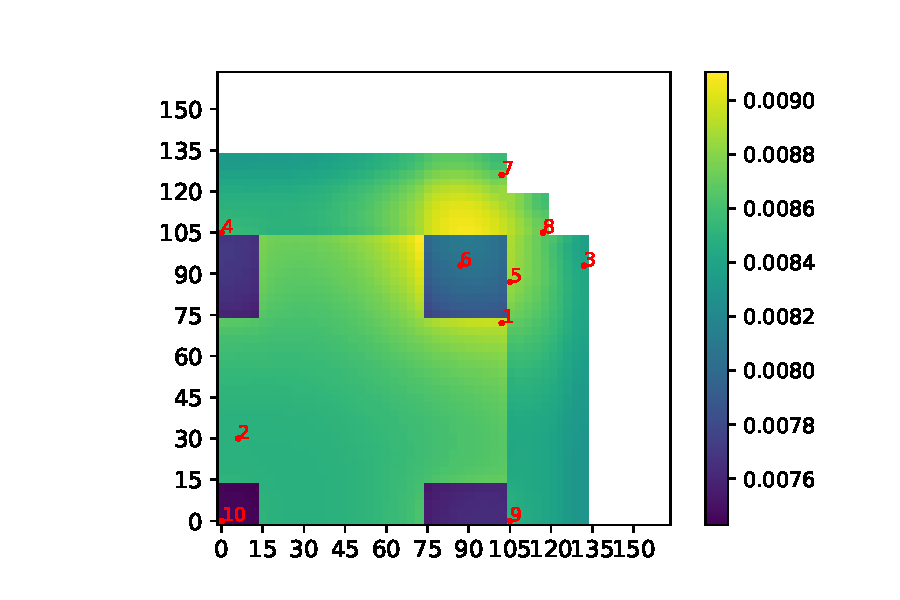
\includegraphics[width=1.0\linewidth]{../figures/LRA_XS_interpolation_points_XS_map.pdf}
	\caption{The fast cross section at t=3 with the selected interpolation indices in red color.}
	\label{fig:cross section deim indices}
\end{figure} 

The power assembly relative errors are computed and shown in Fig.~\ref{fig:assembly power error fm=5} for the $55\times 55$ grid.
The same errors for the other two grids are given in appendix?.
\begin{figure}[H]
	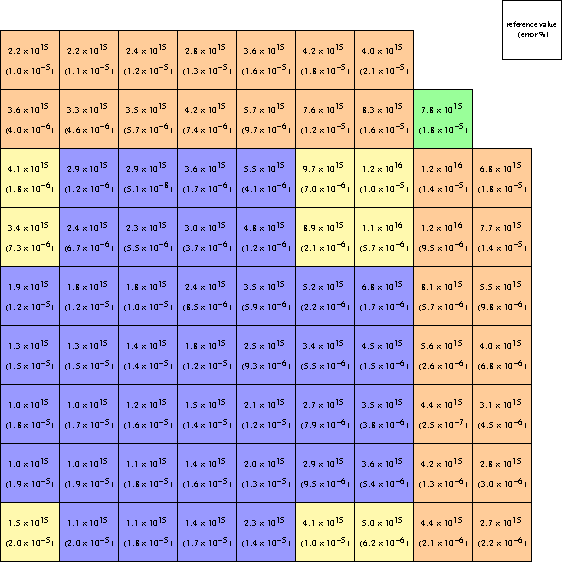
\includegraphics[width=0.9\linewidth]{../figures/lra_assemb_fm=5.pdf}
	\caption{Assembley power relative error for the $55\times 55$ grid}
	\label{fig:assembly power error fm=5}
\end{figure} 

The computational time for the FOM and the ROMS are given in Table~\ref{table:cpu time}.

\begin{table*}[h!]
	\centering
	\caption{\bf computational time of the FOM and the ROMs}
	\label{table:cpu time}
	\begin{tabular}{c|c|c|c}  
		grid &	FOM (s)   &  ROM (s) & MDEIM-ROM (s)    \\
		\hline
		$22\times 22$ & 426   & 140   & 101   \\
		$44\times 44$ &  1652  &   283 &  106  \\
		$55\times 55$ &  2539  & 398   & 110   \\
		\hline
	\end{tabular}
\end{table*}

\section{Using the \texttt{interact} class file}

For convenience, simply copy the \texttt{interact.cls} file into the same directory as your manuscript files (you do not need to install it in your \TeX\ distribution). In order to use the \texttt{interact} document class, replace the command \verb"\documentclass{article}" at the beginning of your document with the command \verb"\documentclass{interact}".

The following document-class options should \emph{not} be used with the \texttt{interact} class file:
\begin{itemize}
  \item \texttt{10pt}, \texttt{11pt}, \texttt{12pt} -- unavailable;
  \item \texttt{oneside}, \texttt{twoside} -- not necessary, \texttt{oneside} is the default;
  \item \texttt{leqno}, \texttt{titlepage} -- should not be used;
  \item \texttt{twocolumn} -- should not be used (see Subsection~\ref{class});
  \item \texttt{onecolumn} -- not necessary as it is the default style.
\end{itemize}
To prepare a manuscript for a journal that is printed in A4 (two column) format, use the \verb"largeformat" document-class option provided by \texttt{interact.cls}; otherwise the class file produces pages sized for B5 (single column) format by default. The \texttt{geometry} package should not be used to make any further adjustments to the page dimensions.

%If your manuscript has supplementary content you can also use the \verb"interact" class file to prepare all or part of it using the \verb"suppldata" document-class option, which will suppress the `article history' date. This option \emph{must not} be used on any primary content. Note that authors are solely responsible for the preparation of all supplemental material.


\section{Additional features of the \texttt{interact} class file}

\subsection{Title, authors' names and affiliations, abstracts and article types}

The title should be generated at the beginning of your article using the \verb"\maketitle" command.
In the final version the author name(s) and affiliation(s) must be followed immediately by \verb"\maketitle" as shown below in order for them to be displayed in your PDF document.
To prepare an anonymous version for double-blind peer review, you can put the \verb"\maketitle" between the \verb"\title" and the \verb"\author" in order to hide the author name(s) and affiliation(s) temporarily.
Next you should include the abstract if your article has one, enclosed within an \texttt{abstract} environment.
The \verb"\articletype" command is also provided as an \emph{optional} element which should \emph{only} be included if your article actually needs it.
For example, the titles for this document begin as follows:
\begin{verbatim}
\articletype{ARTICLE TEMPLATE}

\title{Taylor \& Francis \LaTeX\ template for authors (\textsf{Interact}
layout + NLM reference style)}

\author{
\name{A.~N. Author\textsuperscript{a}\thanks{CONTACT A.~N. Author.
Email: latex.helpdesk@tandf.co.uk} and John Smith\textsuperscript{b}}
\affil{\textsuperscript{a}Taylor \& Francis, 4 Park Square, Milton
Park, Abingdon, UK; \textsuperscript{b}Institut f\"{u}r Informatik,
Albert-Ludwigs-Universit\"{a}t, Freiburg, Germany} }

\maketitle

\begin{abstract}
This template is for authors who are preparing a manuscript for a
Taylor \& Francis journal using the \LaTeX\ document preparation system
and the \texttt{interact} class file, which is available via selected
journals' home pages on the Taylor \& Francis website.
\end{abstract}
\end{verbatim}

An additional abstract in another language (preceded by a translation of the article title) may be included within the \verb"abstract" environment if required.

A graphical abstract may also be included if required. Within the \verb"abstract" environment you can include the code
\begin{verbatim}
\\\resizebox{25pc}{!}{\includegraphics{abstract.eps}}
\end{verbatim}
where the graphical abstract is to appear, where \verb"abstract.eps" is the name of the file containing the graphic (note that \verb"25pc" is the recommended maximum width, expressed in pica, for the graphical abstract in your manuscript).


\subsection{Abbreviations}

A list of abbreviations may be included if required, enclosed within an \texttt{abbreviations} environment, i.e.\ \verb"\begin{abbreviations}"\ldots\verb"\end{abbreviations}", immediately following the \verb"abstract" environment.


\subsection{Keywords}

A list of keywords may be included if required, enclosed within a \texttt{keywords} environment, i.e.\ \verb"\begin{keywords}"\ldots\verb"\end{keywords}". Additional keywords in other languages (preceded by a translation of the word `keywords') may also be included within the \verb"keywords" environment if required.


\subsection{Subject classification codes}

AMS, JEL or PACS classification codes may be included if required. The \texttt{interact} class file provides an \texttt{amscode} environment, i.e.\ \verb"\begin{amscode}"\ldots\verb"\end{amscode}", a \texttt{jelcode} environment, i.e.\ \verb"\begin{jelcode}"\ldots\verb"\end{jelcode}", and a \texttt{pacscode} environment, i.e.\ \verb"\begin{pacscode}"\ldots\verb"\end{pacscode}" to assist with this.


\subsection{Additional footnotes to the title or authors' names}

The \verb"\thanks" command may be used to create additional footnotes to the title or authors' names if required. Footnote symbols for this purpose should be used in the order
$^\ast$~(coded as \verb"$^\ast$"), $\dagger$~(\verb"$\dagger$"), $\ddagger$~(\verb"$\ddagger$"), $\S$~(\verb"$\S$"), $\P$~(\verb"$\P$"), $\|$~(\verb"$\|$"),
$\dagger\dagger$~(\verb"$\dagger\dagger$"), $\ddagger\ddagger$~(\verb"$\ddagger\ddagger$"), $\S\S$~(\verb"$\S\S$"), $\P\P$~(\verb"$\P\P$").

Note that any \verb"footnote"s to the main text will automatically be assigned the superscript symbols 1, 2, 3, etc. by the class file.\footnote{If preferred, the \texttt{endnotes} package may be used to set the notes at the end of your text, before the bibliography. The symbols will be changed to match the style of the journal if necessary by the typesetter.}


\section{Some guidelines for using the standard features of \LaTeX}

\subsection{Sections}

The \textsf{Interact} layout style allows for five levels of section heading, all of which are provided in the \texttt{interact} class file using the standard \LaTeX\ commands \verb"\section", \verb"\subsection", \verb"\subsubsection", \verb"\paragraph" and \verb"\subparagraph". Numbering will be automatically generated for all these headings by default.


\subsection{Lists}

Numbered lists are produced using the \texttt{enumerate} environment, which will number each list item with arabic numerals by default. For example,
\begin{enumerate}
  \item first item
  \item second item
  \item third item
\end{enumerate}
was produced by
\begin{verbatim}
\begin{enumerate}
  \item first item
  \item second item
  \item third item
\end{enumerate}
\end{verbatim}
Alternative numbering styles can be achieved by inserting an optional argument in square brackets to each \verb"item", e.g.\ \verb"\item[(i)] first item"\, to create a list numbered with roman numerals at level one.

Bulleted lists are produced using the \texttt{itemize} environment. For example,
\begin{itemize}
  \item First bulleted item
  \item Second bulleted item
  \item Third bulleted item
\end{itemize}
was produced by
\begin{verbatim}
\begin{itemize}
  \item First bulleted item
  \item Second bulleted item
  \item Third bulleted item
\end{itemize}
\end{verbatim}


\subsection{Figures}

The \texttt{interact} class file will deal with positioning your figures in the same way as standard \LaTeX. It should not normally be necessary to use the optional \texttt{[htb]} location specifiers of the \texttt{figure} environment in your manuscript; you may, however, find the \verb"[p]" placement option or the \verb"endfloat" package useful if a journal insists on the need to separate figures from the text.

Figure captions appear below the figures themselves, therefore the \verb"\caption" command should appear after the body of the figure. For example, Figure~\ref{sample-figure} with caption and sub-captions is produced using the following commands:
\begin{verbatim}
\begin{figure}
\centering
\subfloat[An example of an individual figure sub-caption.]{%
\resizebox*{5cm}{!}{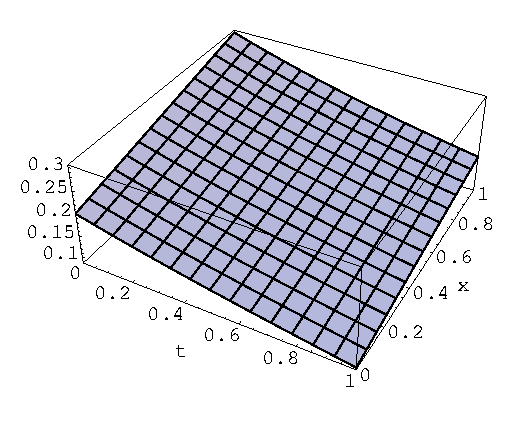
\includegraphics{graph1.eps}}}\hspace{5pt}
\subfloat[A slightly shorter sub-caption.]{%
\resizebox*{5cm}{!}{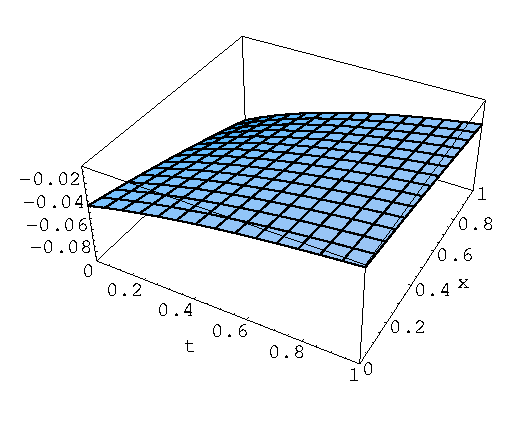
\includegraphics{graph2.eps}}}
\caption{Example of a two-part figure with individual sub-captions
 showing that captions are flush left and justified if greater
 than one line of text.} \label{sample-figure}
\end{figure}
\end{verbatim}
\begin{figure}
\centering
\subfloat[An example of an individual figure sub-caption.]{%
\resizebox*{5cm}{!}{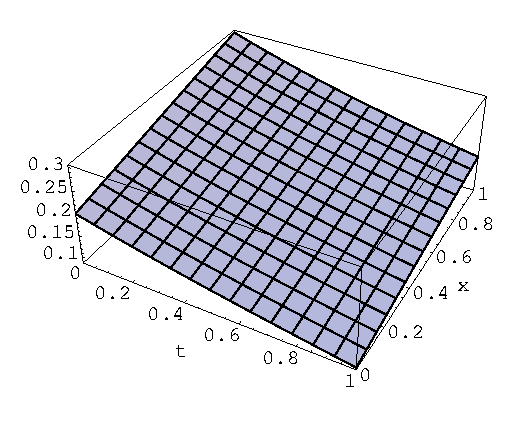
\includegraphics{graph1.eps}}}\hspace{5pt}
\subfloat[A slightly shorter sub-caption.]{%
\resizebox*{5cm}{!}{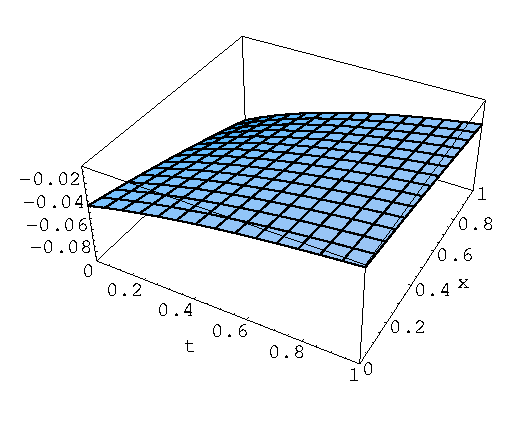
\includegraphics{graph2.eps}}}
\caption{Example of a two-part figure with individual sub-captions
 showing that captions are flush left and justified if greater
 than one line of text.} \label{sample-figure}
\end{figure}

To ensure that figures are correctly numbered automatically, the \verb"\label" command should be included just after the \verb"\caption" command, or in its argument.

The \verb"\subfloat" command requires \verb"subfig.sty", which is called in the preamble of the \texttt{interactnlmsample.tex} file (to allow your choice of an alternative package if preferred) and included in the \textsf{Interact} \LaTeX\ bundle for convenience. Please supply any additional figure macros used with your article in the preamble of your .tex file.

The source files of any figures will be required when the final, revised version of a manuscript is submitted. Authors should ensure that these are suitable (in terms of lettering size, etc.) for the reductions they envisage.

The \texttt{epstopdf} package can be used to incorporate encapsulated PostScript (.eps) illustrations when using PDF\LaTeX, etc. Please provide the original .eps source files rather than the generated PDF images of those illustrations for production purposes.


\subsection{Tables}

The \texttt{interact} class file will deal with positioning your tables in the same way as standard \LaTeX. It should not normally be necessary to use the optional \texttt{[htb]} location specifiers of the \texttt{table} environment in your manuscript; you may, however, find the \verb"[p]" placement option or the \verb"endfloat" package useful if a journal insists on the need to separate tables from the text.

The \texttt{tabular} environment can be used as shown to create tables with single horizontal rules at the head, foot and elsewhere as appropriate. The captions appear above the tables in the \textsf{Interact} style, therefore the \verb"\tbl" command should be used before the body of the table. For example, Table~\ref{sample-table} is produced using the following commands:
\begin{table}
\tbl{Example of a table showing that its caption is as wide as
 the table itself and justified.}
{\begin{tabular}{lcccccc} \toprule
 & \multicolumn{2}{l}{Type} \\ \cmidrule{2-7}
 Class & One & Two & Three & Four & Five & Six \\ \midrule
 Alpha\textsuperscript{a} & A1 & A2 & A3 & A4 & A5 & A6 \\
 Beta & B2 & B2 & B3 & B4 & B5 & B6 \\
 Gamma & C2 & C2 & C3 & C4 & C5 & C6 \\ \bottomrule
\end{tabular}}
\tabnote{\textsuperscript{a}This footnote shows how to include
 footnotes to a table if required.}
\label{sample-table}
\end{table}
\begin{verbatim}
\begin{table}
\tbl{Example of a table showing that its caption is as wide as
 the table itself and justified.}
{\begin{tabular}{lcccccc} \toprule
 & \multicolumn{2}{l}{Type} \\ \cmidrule{2-7}
 Class & One & Two & Three & Four & Five & Six \\ \midrule
 Alpha\textsuperscript{a} & A1 & A2 & A3 & A4 & A5 & A6 \\
 Beta & B2 & B2 & B3 & B4 & B5 & B6 \\
 Gamma & C2 & C2 & C3 & C4 & C5 & C6 \\ \bottomrule
\end{tabular}}
\tabnote{\textsuperscript{a}This footnote shows how to include
 footnotes to a table if required.}
\label{sample-table}
\end{table}
\end{verbatim}

To ensure that tables are correctly numbered automatically, the \verb"\label" command should be included just before \verb"\end{table}".

The \verb"\toprule", \verb"\midrule", \verb"\bottomrule" and \verb"\cmidrule" commands are those used by \verb"booktabs.sty", which is called by the \texttt{interact} class file and included in the \textsf{Interact} \LaTeX\ bundle for convenience. Tables produced using the standard commands of the \texttt{tabular} environment are also compatible with the \texttt{interact} class file.


\subsection{Landscape pages}

If a figure or table is too wide to fit the page it will need to be rotated, along with its caption, through 90$^{\circ}$ anticlockwise. Landscape figures and tables can be produced using the \verb"rotating" package, which is called by the \texttt{interact} class file. The following commands (for example) can be used to produce such pages.
\begin{verbatim}
\setcounter{figure}{1}
\begin{sidewaysfigure}
\centerline{\epsfbox{figname.eps}}
\caption{Example landscape figure caption.}
\label{landfig}
\end{sidewaysfigure}
\end{verbatim}
\begin{verbatim}
\setcounter{table}{1}
\begin{sidewaystable}
 \tbl{Example landscape table caption.}
  {\begin{tabular}{@{}llllcll}
    .
    .
    .
  \end{tabular}}\label{landtab}
\end{sidewaystable}
\end{verbatim}
Before any such float environment, use the \verb"\setcounter" command as above to fix the numbering of the caption (the value of the counter being the number given to the preceding figure or table). Subsequent captions will then be automatically renumbered accordingly. The \verb"\epsfbox" command requires \verb"epsfig.sty", which is called by the \texttt{interact} class file and is also included in the \textsf{Interact} \LaTeX\ bundle for convenience.

Note that if the \verb"endfloat" package is used, one or both of the commands
\begin{verbatim}
\DeclareDelayedFloatFlavor{sidewaysfigure}{figure}
\DeclareDelayedFloatFlavor{sidewaystable}{table}
\end{verbatim}
will need to be included in the preamble of your .tex file, after the \verb"endfloat" package is loaded, in order to process any landscape figures and/or tables correctly.


\subsection{Theorem-like structures}

A predefined \verb"proof" environment is provided by the \texttt{amsthm} package (which is called by the \texttt{interact} class file), as follows:
\begin{proof}
More recent algorithms for solving the semidefinite programming relaxation are particularly efficient, because they explore the structure of the MAX-CUT problem.
\end{proof}
\noindent This was produced by simply typing:
\begin{verbatim}
\begin{proof}
More recent algorithms for solving the semidefinite programming
relaxation are particularly efficient, because they explore the
structure of the MAX-CUT problem.
\end{proof}
\end{verbatim}
Other theorem-like environments (theorem, definition, remark, etc.) need to be defined as required, e.g.\ using \verb"\newtheorem{theorem}{Theorem}" in the preamble of your .tex file (see the preamble of \verb"interactnlmsample.tex" for more examples). You can define the numbering scheme for these structures however suits your article best. Please note that the format of the text in these environments may be changed if necessary to match the style of individual journals by the typesetter during preparation of the proofs.


\subsection{Mathematics}

\subsubsection{Displayed mathematics}

The \texttt{interact} class file will set displayed mathematical formulas centred on the page without equation numbers if you use the \texttt{displaymath} environment or the equivalent \verb"\[...\]" construction. For example, the equation
\[
 \hat{\theta}_{w_i} = \hat{\theta}(s(t,\mathcal{U}_{w_i}))
\]
was typeset using the commands
\begin{verbatim}
\[
 \hat{\theta}_{w_i} = \hat{\theta}(s(t,\mathcal{U}_{w_i}))
\]
\end{verbatim}

For those of your equations that you wish to be automatically numbered sequentially throughout the text for future reference, use the \texttt{equation} environment, e.g.
\begin{equation}
 \hat{\theta}_{w_i} = \hat{\theta}(s(t,\mathcal{U}_{w_i}))
\end{equation}
was typeset using the commands
\begin{verbatim}
\begin{equation}
 \hat{\theta}_{w_i} = \hat{\theta}(s(t,\mathcal{U}_{w_i}))
\end{equation}
\end{verbatim}

Part numbers for sets of equations may be generated using the \texttt{subequations} environment, e.g.
\begin{subequations} \label{subeqnexample}
\begin{equation}
     \varepsilon \rho w_{tt}(s,t) = N[w_{s}(s,t),w_{st}(s,t)]_{s},
     \label{subeqnparta}
\end{equation}
\begin{equation}
     w_{tt}(1,t)+N[w_{s}(1,t),w_{st}(1,t)] = 0,   \label{subeqnpartb}
\end{equation}
\end{subequations}
which was typeset using the commands
\begin{verbatim}
\begin{subequations} \label{subeqnexample}
\begin{equation}
     \varepsilon \rho w_{tt}(s,t) = N[w_{s}(s,t),w_{st}(s,t)]_{s},
     \label{subeqnparta}
\end{equation}
\begin{equation}
     w_{tt}(1,t)+N[w_{s}(1,t),w_{st}(1,t)] = 0,   \label{subeqnpartb}
\end{equation}
\end{subequations}
\end{verbatim}
This is made possible by the \texttt{amsmath} package, which is called by the class file. If you put a \verb"\label" just after the \verb"\begin{subequations}" command, references can be made to the collection of equations, i.e.\ `(\ref{subeqnexample})' in the example above. Or, as the example also shows, you can label and refer to each equation individually -- i.e.\ `(\ref{subeqnparta})' and `(\ref{subeqnpartb})'.

Displayed mathematics should be given end-of-line punctuation appropriate to the running text sentence of which it forms a part, if required.

\subsubsection{Math fonts}

\paragraph{Superscripts and subscripts}
Superscripts and subscripts will automatically come out in the correct size in a math environment (i.e.\ enclosed within \verb"\(...\)" or \verb"$...$" commands in running text, or within \verb"\[...\]" or the \texttt{equation} environment for displayed equations). Sub/superscripts that are physical variables should be italic, whereas those that are labels should be roman (e.g.\ $C_p$, $T_\mathrm{eff}$). If the subscripts or superscripts need to be other than italic, they must be coded individually.

\paragraph{Upright Greek characters and the upright partial derivative sign}
Upright lowercase Greek characters can be obtained by inserting the letter `u' in the control code for the character, e.g.\ \verb"\umu" and \verb"\upi" produce $\umu$ (used, for example, in the symbol for the unit microns -- $\umu\mathrm{m}$) and $\upi$ (the ratio of the circumference of a circle to its diameter). Similarly, the control code for the upright partial derivative $\upartial$ is \verb"\upartial". Bold lowercase as well as uppercase Greek characters can be obtained by \verb"{\bm \gamma}", for example, which gives ${\bm \gamma}$, and \verb"{\bm \Gamma}", which gives ${\bm \Gamma}$.


\section*{Acknowledgement(s)}

An unnumbered section, e.g.\ \verb"\section*{Acknowledgements}", may be used for thanks, etc.\ if required and included \emph{in the non-anonymous version} before any Notes or References.


\section*{Disclosure statement}

An unnumbered section, e.g.\ \verb"\section*{Disclosure statement}", may be used to declare any potential conflict of interest and included \emph{in the non-anonymous version} before any Notes or References, after any Acknowledgements and before any Funding information.


\section*{Funding}

An unnumbered section, e.g.\ \verb"\section*{Funding}", may be used for grant details, etc.\ if required and included \emph{in the non-anonymous version} before any Notes or References.


\section*{Notes on contributor(s)}

An unnumbered section, e.g.\ \verb"\section*{Notes on contributors}", may be included \emph{in the non-anonymous version} if required. A photograph may be added if requested.


\section*{Nomenclature/Notation}

An unnumbered section, e.g.\ \verb"\section*{Nomenclature}" (or \verb"\section*{Notation}"), may be included if required, before any Notes or References.


\section*{Notes}

An unnumbered `Notes' section may be included before the References (if using the \verb"endnotes" package, use the command \verb"\theendnotes" where the notes are to appear, instead of creating a \verb"\section*").


\section{References}

\subsection{References cited in the text}

References should be cited in accordance with US National Library of Medicine (NLM) style. References are cited in the text by a number in square brackets (e.g. [1], [2,4,10], [11--15], \emph{not} [11]--[15]), in the order in which they first appear. For further details on this reference style, see the Instructions for Authors on the Taylor \& Francis website.

Each bibliographic entry has a key, which is assigned by the author and is used to refer to that entry in the text. In this document, the key \verb"Jen05" in the citation form \verb"\cite{Jen05}" produces `\cite{Jen05}', and the keys \verb"{Sch02,Wen95}" in the citation form \verb"\cite{Sch02,Wen95}" produce `\cite{Sch02,Wen95}'. The citation for a range of bibliographic entries (e.g.\ `\cite{Sha78,AG98,Smi75,Men05,DCK03,Hor98,Ant03,Zha05,Rog05,SRW05}') will automatically be produced by  \verb"\cite{Sha78,AG98,Smi75,Men05,DCK03,Hor98,Ant03,Zha05,Rog05,SRW05}". Optional notes may be included at the beginning and/or end of a citation by the use of square brackets, e.g.\ \verb"\cite[cf.][]{Gau05}" produces `\cite[cf.][]{Gau05}', \verb"\cite[p.356]{BGC04}" produces `\cite[p.356]{BGC04}', and \verb"\cite[see][p.73-–77]{PI51}" produces `\cite[see][p.73--77]{PI51}'.


\subsection{The list of references}

References should be listed at the end of the main text in the order in which they are first cited in the text. The following list shows some sample references prepared in the Taylor \& Francis NLM style.

\begin{thebibliography}{99}

\bibitem{Jen05}%1
Jenkins~PF. Making sense of the chest x-ray: a hands-on guide. New York (NY):
  Oxford University Press; 2005.

\bibitem{Sch02}%2
Schott~J, Priest~J. Leading antenatal classes: a practical guide. 2nd ed.
  Boston (MA): Books for Midwives; 2002.

\bibitem{Wen95}%3
Wenger~NK, Sivarajan~Froelicher~E, Smith~LK, et~al. Cardiac rehabilitation.
  Rockville (MD): Agency for Health Care Policy and Research (US); 1995.

\bibitem{Sha78}%4
Shakelford~RT. Surgery of the alimentary tract. Philadelphia (PA): W.B.
  Saunders; 1978. Chapter 2, Esophagoscopy; p. 29--40.

\bibitem{AG98}%5
Ambudkar~SV, Gottesman~MM, editors. {ABC} transporters: biomedical, cellular,
  and molecular aspects. San Diego (CA): Academic Press; 1998. (Methods in
  enzymology; vol. 292).

\bibitem{Smi75}%6
Smith~CE. The significance of mosquito longevity and blood-feeding behaviour in
  the dynamics of arbovirus infections. Med Biol. 1975;53:288--294.

\bibitem{Men05}%7
Meneton~P, Jeunemaitre~X, de~Wardener~HE, et~al. Links between dietary salt
  intake, renal salt handling, blood pressure, and cardiovascular diseases.
  Physiol Rev. 2005 Apr;85:679--715.

\bibitem{DCK03}%8
Dostorovsky~JO, Carr~DB, Koltzenburg~M, editors. Proceedings of the 10th World
  Congress on Pain; 2002 Aug~17--22; San Diego, CA. Seattle: IASP Press; c2003.

\bibitem{Hor98}%9
Horrobin~DF, Lampinskas~P. The commercial development of food plants used as
  medicines. In: Prendergast~HD, Etkin~NL, Harris~DR, et~al., editors. Plants
  for food and medicine. Proceedings of the Joint Conference of the Society for
  Economic Botany and the International Society for Ethnopharmacology; 1996
  Jul~1--6; London. Kew (UK): Royal Botanic Gardens; 1998. p. 75--81.

\bibitem{Ant03}%10
Antani~S, Long~LR, Thoma~GR, et~al. Anatomical shape representation in spine
  x-ray images. Paper presented at: VIIP 2003. Proceedings of the 3rd IASTED
  International Conference on Visualization, Imaging and Image Processing;
  2003 Sep~8--10; Benalmadena, Spain.

\bibitem{Zha05}%11
Zhao~C. Development of nanoelectrospray and application to protein research and
  drug discovery [dissertation]. Buffalo (NY): State University of New York at
  Buffalo; 2005.

\bibitem{Rog05}%12
Roguskie~JM. The role of \emph{Pseudomonas aeruginosa} 1244 pilin glycan in
  virulence [master's thesis]. [Pittsburgh (PA)]: Duquesne University; 2005.

\bibitem{SRW05}%13
Savage~E, Ramsay~M, White~J, et~al. Mumps outbreaks across England and Wales
  in 2004: Observational study. BMJ. 2005;330(7500):1119--1120 [cited 2005
  May~31]; Available from: http://bmj.bmjjournals.com/cgi/reprint/330/7500/1119.

\bibitem{Gau05}%14
Gaul~G. When geography influences treament options. Washington Post (Maryland
  Ed.). 2005 Jul~24;Sect.~A:12 (col.~1).

\bibitem{BGC04}%15
Berrino~F, Gatta~G, Crosignani~P. [Case-control evaluation of screening
  efficacy]. Epidemiol Prev. 2004 Nov--Dec;28:354--359. Italian.

\bibitem{PI51}%16
Piaget~J, Inhelder~B. La gen{\`e}se de l'id{\'e}e de hasard chez l'enfant
  [The origin of the idea of chance in the child]. Paris: Presses
  Universitaires de France; 1951.

\end{thebibliography}
\bigskip
\noindent This was produced by typing:
\begin{verbatim}
\begin{thebibliography}{99}

\bibitem{Jen05}%1
Jenkins~PF. Making sense of the chest x-ray: a hands-on guide. New York
 (NY): Oxford University Press; 2005.

\bibitem{Sch02}%2
Schott~J, Priest~J. Leading antenatal classes: a practical guide. 2nd
 ed. Boston (MA): Books for Midwives; 2002.

\bibitem{Wen95}%3
Wenger~NK, Sivarajan~Froelicher~E, Smith~LK, et~al. Cardiac
 rehabilitation. Rockville (MD): Agency for Health Care Policy and
 Research (US); 1995.

\bibitem{Sha78}%4
Shakelford~RT. Surgery of the alimentary tract. Philadelphia (PA):
 W.B. Saunders; 1978. Chapter 2, Esophagoscopy; p. 29--40.

\bibitem{AG98}%5
Ambudkar~SV, Gottesman~MM, editors. {ABC} transporters: biomedical,
 cellular, and molecular aspects. San Diego (CA): Academic Press; 1998.
 (Methods in enzymology; vol. 292).

\bibitem{Smi75}%6
Smith~CE. The significance of mosquito longevity and blood-feeding
 behaviour in the dynamics of arbovirus infections. Med Biol.
 1975;53:288--294.

\bibitem{Men05}%7
Meneton~P, Jeunemaitre~X, de~Wardener~HE, et~al. Links between dietary
 salt intake, renal salt handling, blood pressure, and cardiovascular
 diseases. Physiol Rev. 2005 Apr;85:679--715.

\bibitem{DCK03}%8
Dostorovsky~JO, Carr~DB, Koltzenburg~M, editors. Proceedings of the
 10th World Congress on Pain; 2002 Aug~17--22; San Diego, CA. Seattle:
 IASP Press; c2003.

\bibitem{Hor98}%9
Horrobin~DF, Lampinskas~P. The commercial development of food plants
 used as medicines. In: Prendergast~HD, Etkin~NL, Harris~DR, et~al.,
 editors. Plants for food and medicine. Proceedings of the Joint
 Conference of the Society for Economic Botany and the International
 Society for Ethnopharmacology; 1996 Jul~1--6; London. Kew (UK): Royal
 Botanic Gardens; 1998. p. 75--81.

\bibitem{Ant03}%10
Antani~S, Long~LR, Thoma~GR, et~al. Anatomical shape representation in
 spine x-ray images. Paper presented at: VIIP 2003. Proceedings of the
 3rd IASTED International Conference on Visualization, Imaging and
 Image Processing; 2003 Sep~8--10; Benalmadena, Spain.

\bibitem{Zha05}%11
Zhao~C. Development of nanoelectrospray and application to protein
 research and drug discovery [dissertation]. Buffalo (NY): State
 University of New York at Buffalo; 2005.

\bibitem{Rog05}%12
Roguskie~JM. The role of \emph{Pseudomonas aeruginosa} 1244 pilin
 glycan in virulence [master's thesis]. [Pittsburgh (PA)]: Duquesne
 University; 2005.

\bibitem{SRW05}%13
Savage~E, Ramsay~M, White~J, et~al. Mumps outbreaks across England and
 Wales in 2004: Observational study. BMJ. 2005;330(7500):1119--1120
 [cited 2005 May 31]; Available from:
 http://bmj.bmjjournals.com/cgi/reprint/330/7500/1119.

\bibitem{Gau05}%14
Gaul~G. When geography influences treament options. Washington Post
 (Maryland Ed.). 2005 Jul~24;Sect.~A:12 (col.~1).

\bibitem{BGC04}%15
Berrino~F, Gatta~G, Crosignani~P. [Case-control evaluation of screening
 efficacy]. Epidemiol Prev. 2004 Nov--Dec;28:354--359. Italian.

\bibitem{PI51}%16
Piaget~J, Inhelder~B. La gen{\`e}se de l'id{\'e}e de hasard chez
 l'enfant [The origin of the idea of chance in the child]. Paris:
 Presses Universitaires de France; 1951.

\end{thebibliography}
\end{verbatim}
\bigskip
\noindent Each entry takes the form:
\begin{verbatim}
\bibitem{key}%n Bibliography entry
\end{verbatim}
where `\texttt{key}' is the tag that is to be used as an argument for the \verb"\cite{}" commands in the text of the article and `\texttt{Bibliography entry}' is the material that is to appear in the list of references, suitably formatted. The commands
\begin{verbatim}
\usepackage[numbers,sort&compress]{natbib}
\bibpunct[, ]{[}{]}{,}{n}{,}{,}
\renewcommand\bibfont{\fontsize{10}{12}\selectfont}
\makeatletter
\def\NAT@def@citea{\def\@citea{\NAT@separator}}
\makeatother
\end{verbatim}
need to be included in the preamble of your .tex file in order to generate the citations and bibliography as described above.

Instead of typing the bibliography by hand, you may prefer to create the list of references using a \textsc{Bib}\TeX\ database. The \texttt{tfnlm.bst} file needs to be in your working folder or an appropriate directory, and the lines
\begin{verbatim}
\bibliographystyle{tfnlm}
\bibliography{interactnlmsample}
\end{verbatim}
included where the list of references is to appear, where \texttt{tfnlm.bst} is the name of the \textsc{Bib}\TeX\ bibliography style file for Taylor \& Francis' NLM reference style and \texttt{interactnlmsample.bib} is the bibliographic database included with the \textsf{Interact}-NLM \LaTeX\ bundle (to be replaced with the name of your own .bib file). \LaTeX/\textsc{Bib}\TeX\ will extract from your .bib file only those references that are cited in your .tex file and list them in the References section.

Please include a copy of your .bib file and/or the final generated .bbl file among your source files if your .tex file does not contain a reference list in a \texttt{thebibliography} environment.


\section{Appendices}

Any appendices should be placed after the list of references, beginning with the command \verb"\appendix" followed by the command \verb"\section" for each appendix title, e.g.
\begin{verbatim}
\appendix
\section{This is the title of the first appendix}
\section{This is the title of the second appendix}
\end{verbatim}
produces:\medskip

\noindent\textbf{Appendix A. This is the title of the first appendix}\medskip

\noindent\textbf{Appendix B. This is the title of the second appendix}\medskip

\noindent Subsections, equations, figures, tables, etc.\ within appendices will then be automatically numbered as appropriate. Some theorem-like environments may need to have their counters reset manually (e.g.\ if they are not numbered within sections in the main text). You can achieve this by using \verb"\numberwithin{remark}{section}" (for example) just after the \verb"\appendix" command.

Note that if the \verb"endfloat" package is used on a document containing any appendices, the \verb"\processdelayedfloats" command must be included immediately before the \verb"\appendix" command in order to ensure that the floats belonging to the main body of the text are numbered as such.

%\processdelayedfloats %%% See above for an explanation of why this command might be needed here.

\appendix

\section{Troubleshooting}

Authors may occasionally encounter problems with the preparation of a manuscript using \LaTeX. The appropriate action to take will depend on the nature of the problem:
\begin{enumerate}
\item[(i)] If the problem is with \LaTeX\ itself, rather than with the actual macros, please consult an appropriate \LaTeXe\ manual for initial advice. If the solution cannot be found, or if you suspect that the problem does lie with the macros, then please contact Taylor \& Francis for assistance (\texttt{latex.helpdesk@tandf.co.uk}), clearly stating the title of the journal to which you are submitting.
\item[(ii)] Problems with page make-up (e.g.\ occasional overlong lines of text; figures or tables appearing out of order): please do not try to fix these using `hard' page make-up commands -- the typesetter will deal with such problems. (You may, if you wish, draw attention to particular problems when submitting the final version of your manuscript.)
\item[(iii)] If a required font is not available on your system, allow \TeX\ to substitute the font and specify which font is required in a covering letter accompanying your files.
\end{enumerate}


\section{Obtaining the template and class file}

\subsection{Via the Taylor \& Francis website}

This article template and the \texttt{interact} class file may be obtained via the `Instructions for Authors' pages of selected Taylor \& Francis journals.

Please note that the class file calls up the open-source \LaTeX\ packages booktabs.sty, epsfig.sty and rotating.sty, which will, for convenience, unpack with the downloaded template and class file. The template calls for natbib.sty and subfig.sty, which are also supplied for convenience.


\subsection{Via e-mail}

This article template, the \texttt{interact} class file and the associated open-source \LaTeX\ packages are also available via e-mail. Requests should be addressed to \texttt{latex.helpdesk@tandf.co.uk}, clearly stating for which journal you require the template and class file.

\end{document}
